% Chapter 1

\chapter{Sound nomenclature} % Main chapter title
\label{Chapter1} % To reference to this chapter elsewhere, use \ref{Chapter1} 
\lhead{Chapter 1. \emph{Sound nomenclature}} % This is for the header on each page - perhaps a shortened title
\textsf{\textsl{Written by Bjorn Deraeve}}
%----------------------------------------------------------------------------------------

\section{Introduction}
Sound is the human perception of little changes in air pressure. This oscillation of pressure, referred to as a sound wave, is a mechanical wave propagated through a solid, liquid or gas and is composed of frequencies within the range of hearing. For humans this is between about 20 Hz and 20 000 Hz, however the upper limit generally decreases with one's age.   The changes in pressure must also be big enough in order to be audible.

The mechanical vibrations interpreted as sound waves are longitudinal waves. Any source makes the matter in the medium periodically displace and thus oscillating. The alternating pressure deviations from the equilibrium pressure are in the same direction as the energy propagation of the wave. The energy carried by the wave is converted between potential energy (extra compression) and kinetic energy (oscillations of the medium).

When a sound wave reaches the eardrum it starts to oscillate at a frequency corresponding to the sound waves frequency. These vibrations are detected by hair cells in the inner ear and are transduced into nerve pulses (action potentials) which transmit information about the sound to the brain.

Sound waves are often described as sinusoidal waves which are characterized by a wavelength and amplitude. The wavelength is directly related to the frequency as $\lambda$ = $\frac{v}{f}$.  The higher the frequency, the higher the perceived tone will be. In dry air the speed of sound is approximately 343 meters per second. 

The sound wave causes a local pressure deviation from the ambient atmospheric pressure. To measure this deviation one uses the sound pressure level (SPL) scale. Since the human ear can detect sounds with a wide range of amplitudes (volumes) it is a logarithmic measure of the sound pressure at the deviation relative to a reference value. It is thus measured in an amount of decibels (dB) above the reference level. SPL is defined as:
\begin{equation}
L_{P} = 10\cdot \mathrm{log}_{10} (\frac{p^{2}}{p_{ref^{2}}} ) = 20 \cdot \mathrm{log}_{10} (\frac{p}{p_{ref}}) \medspace dB
\end{equation}
where p is the rms value of the measured sound pressure and pref is the reference sound pressure, pref = 20 microPa (rms), considered as the threshold of human hearing.
%----------------------------------------------------------------------------------------

\section{Sound characteristics}
A sound is defined by several characteristics. The most important are pitch (dutch: 'toonhoogte'), timbre (dutch: 'klankkleur') and are briefly introduced in this section. Other characteristics are volume and the duration of the rising of the sound, of the persistence and of the damping.
%----------------------------------------------------------------------------------------

\subsection{Pitch and tone}
For the human ear a pure tone is a sound with a constant frequency and timbre. This fundamental frequency, the number of perceived oscillations per second, is called the pitch of the sound. It is the frequency of the lowest tone present in the sound and is directly related to the frequency spectrum of the sound. Pitch allows the ordering of sounds on a frequency-based scale and is determined by the vibration frequency of the air. If air vibrations are not regularly there is no fixed frequency, such sound is called noise. On staves the pitch is indicated by the location of the note on the staff. The heigher the tone the higher the note is positioned on the staff.
\begin{figure}[htbp]
\centering
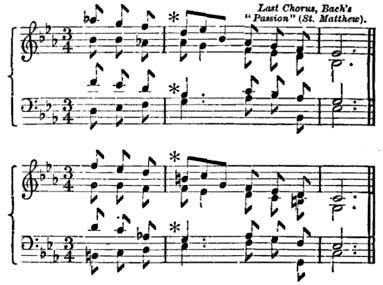
\includegraphics[height=5cm]{staff}
\rule{30em}{0.5pt}
\caption{Position of notes on staves}
\label{fig:staff}
\end{figure} \\
A tone with a double pitch is said to be one octave higher and is the first upper tone. In addition to the ordinary meaning of tone and pitch, in Western music theory tone is also the abstract term of future tones te sound, represented by the letters A to G and derived symbols (A = 440Hz). In some countries the fundamental tones are not indicated by letters but by the Greek diatonic scale (do-re-mi-fa-sol-la-si-do).
%----------------------------------------------------------------------------------------

\subsection{Timbre}
Timbre is the quality of a sound that distinguishes different musical instruments and voices. Timbre or tone colour is determined by the fundamental frequency (pitch) and the present overtones, also known as upper partials or harmonics, so timbre is composed of many different frequency components. It is determined by the ratio of the strength of the overtone vibrations in the sound in proportion to the fundamental frequency  of the sound.  

\subsubsection{Spectral diagram}
At this moment it is interesting to have a look at the spectral diagram of a sound. This diagram provides a link between the aural experience and visual representation of a sound. It does this by representing the energy (loudness, height of the line) and the frequency (position of the line) of the different frequency components within the timbre. It is unique to any sound and gives audible information about that sound. Waveforms are very descriptive for the way air pressure changes with time but not for the actual timbre of a sound.
\begin{figure}[htbp]
\centering
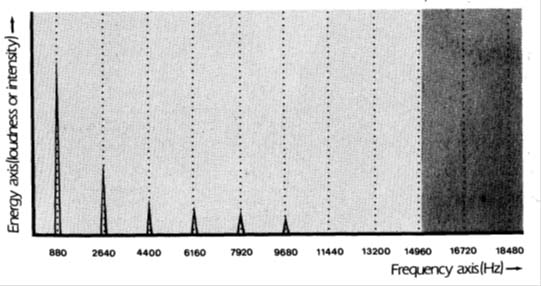
\includegraphics[height=5cm]{spectral}
\rule{30em}{0.5pt}
\caption{Spectral diagram of a timbre}
\label{fig:spectral}
\end{figure} \\
How can we interpret figure \ref{fig:spectral}? The line on the left is the fundamental frequency or first harmonic. The other frequencies visible in the spectrum, on the right of the first harmonic, indicate the other present frequencies in the sound. Most generally those are called 'partials'. If all partials are an integer multiple of the fundamental frequency they are called 'harmonics' or 'overtones' and the sound exists of the 'natural' harmonic frequencies only. \\ As we can see from the spectrum in figure \ref{fig:spectral}, the partials are in the harmonic series. The note played in this figure was A = 880Hz, this is the first harmonic. The next harmonic is at 3 times 880Hz or 2640Hz. This is the third harmonic, and so on. \\  From the relative height of the lines (representing the energy or loudness) we can deduce that the harmonics become weaker.
\subsubsection{Joseph Fourier}
Today when musicians desribe a timbre they talk about overtones, partials or harmonics, but it was the French mathematician and physicist Joseph Fourier who gave a mathematical basis to this idea with his work 'Th\'{e}orie de la chaleur" which he presented in 1822. In this investigation of the use of Fourier series for problems of heat transfer and vibrations, he brought up the following simplified statement: each complex sound, such as that from a violin or trumpet, can be thought of as the sum of a collection of much simpler tones (sines),  at frequencies which are an integer number multiples of the fundamental frequency (pitch). In other words: each complex sound can be resolved into mixtures of sine functions which may differ in amplitude and period but of which all periods are related as an integer multiple. This resolving into different components is called a Fourier transformation or analysis of the signal. \\ The spectrum as in figure \ref{fig:spectral} shows clearly the present frequencies (= partials, overtones or harmonics) and their energy level.
\begin{figure}[htbp]
   \centerline{\hbox{
   \epsfxsize=1.2in
   \epsffile{/fourier.jpg}
     }
  }
  \caption{Sketch of Fourier}
  \label{fig:fourier}
\end{figure}

